% Created 2022-10-18 Tue 14:08
% Intended LaTeX compiler: pdflatex
\documentclass[presentation,aspectratio=169]{beamer}
\usepackage[utf8]{inputenc}
\usepackage[T1]{fontenc}
\usepackage{graphicx}
\usepackage{grffile}
\usepackage{longtable}
\usepackage{wrapfig}
\usepackage{rotating}
\usepackage[normalem]{ulem}
\usepackage{amsmath}
\usepackage{textcomp}
\usepackage{amssymb}
\usepackage{capt-of}
\usepackage{hyperref}
\usepackage{pifont}
\newcommand{\cmark}{\textcolor{green!80!black}{\ding{51}}}
\usepackage{amssymb}
\usepackage{pgfplotstable}
\DeclareMathOperator{\shift}{q}
\DeclareMathOperator{\diff}{p}
\usepackage{khpreamble, euscript, mathtools}
\DeclareMathOperator{\atantwo}{atan2}
\newcommand*{\ctrb}{\EuScript{C}}
\newcommand*{\obsv}{\EuScript{O}}
\usetheme{default}
\author{Kjartan Halvorsen}
\date{\today}
\title{State feedback with observer}
\hypersetup{
 pdfauthor={Kjartan Halvorsen},
 pdftitle={State feedback with observer},
 pdfkeywords={},
 pdfsubject={},
 pdfcreator={Emacs 26.3 (Org mode 9.4.6)}, 
 pdflang={English}}
\begin{document}

\maketitle



\section{State feedback with observer}
\label{sec:org2d43c1c}
\begin{frame}[label={sec:org9c6fdd4}]{State feedback with reconstructed states}
\end{frame}

\begin{frame}[label={sec:org9053424}]{State feedback with reconstructed states}
\begin{center}
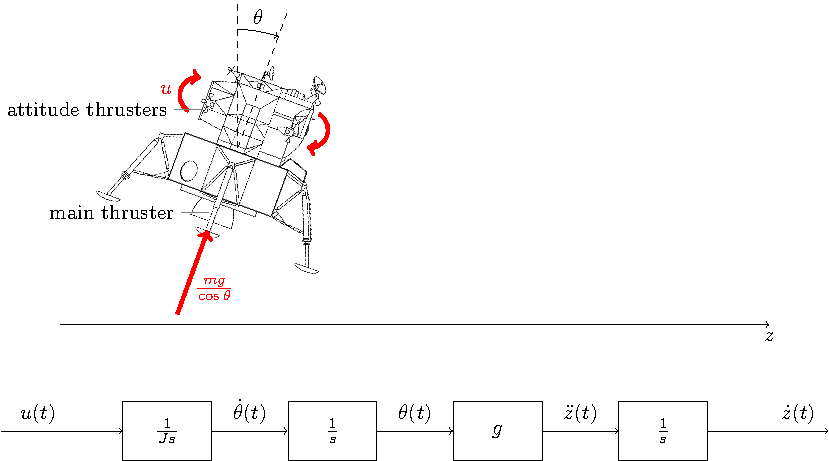
\includegraphics[width=0.9\linewidth]{../../figures/fig-apollo}
\end{center}
\end{frame}

\begin{frame}[label={sec:orgd52a7c0}]{State feedback}
Given
 \begin{equation}
 \begin{split}
  \dot{x} &= A x + B u\\
  y &= C x
 \end{split}
 \label{eq:ssmodel}
\end{equation}
and measurements (or estimates) of the state vector \(x\). 

\alert{Linear state feedback} is the control law
\begin{equation*}
\begin{split}
 u &= f\big((x, u_c\big) = -l_1x_1 - l_2x_2 - \cdots - l_n x_n + l_0u_c\\
      &= -\textcolor{morange}{L}x + l_0u_c, 
\end{split}
\end{equation*}
where \[ \textcolor{morange}{L} = \bbm l_1 & l_2 & \cdots & l_n \ebm. \]
Substituting the control law in the state space model \eqref{eq:ssmodel} gives
 \begin{equation}
 \begin{split}
  \dot{x} &= \left(A -B \textcolor{morange}{L} \right) x + l_0B r\\
  y(k) &= C x
 \end{split}
 \label{eq:closedloop}
\end{equation}
\end{frame}



\begin{frame}[label={sec:org331a250}]{Observer design}
Given model
 \begin{equation*}
 \begin{split}
  \dot{x} &= A x + B u\\
  y &= C x
 \end{split}
 \label{eq:ssmodel}
\end{equation*}
and measurements of the output signal \(y\). 

The observer is given by
\begin{equation*}
\begin{split}
\dot{\hat{x}} &= \underbrace{A \hat{x} + B u{}}_{\text{simulation}} + \underbrace{\textcolor{mred}{K}\big(y - C\hat{x}\big)}_{\text{correction}} = \left(A - \textcolor{mred}{K}C\right)\hat{x} +  B u{} + \textcolor{mred}{K}y
\end{split}
\end{equation*}
with poles given by the eigenvalues of the matrix \(A_o = A - \textcolor{mred}{K}C\)

\alert{Rule-of-thumb} Choose the poles of the observer (eigenvalues of \(A-\textcolor{mred}{K}C\)) at least twice as fast as the poles (eigenvalues) of \(A-B \textcolor{morange}{L}\).
\end{frame}


\begin{frame}[label={sec:orge761c84}]{Control by feedback from reconstructed states}
The design problem can be separated into two problems
\begin{enumerate}
\item Determine the gain vector \(\textcolor{orange!80!black}{L}\) and the gain \(\textcolor{mbluegreen}{l_0}\) of the control law
\[ u{} = -\textcolor{orange!80!black}{L} \hat{x} + \textcolor{mbluegreen}{l_0} r\]
so that the closed-loop system has good reference tracking.
\item Determine the gain vector \(\textcolor{mred}{K}\) of the observer
\begin{equation*}
\begin{split}
\dot{\hat{x}} &= A \hat{x} + B u{} + \textcolor{mred}{K} \big(y - C\hat{x}\big)
\end{split}
\end{equation*}
to get a good balance between disturbance rejection and noise attenuation.
\end{enumerate}
\end{frame}

\begin{frame}[label={sec:org6159338}]{Computing the observer gain}
A matrix \(M\) and its transpose \(M\transp\) have the same eigenvalues. Hence, the problem of determining the gain \(K\) to obtain desired eigenvalues of 
\[A- \textcolor{mred}{K}C\] is equivalent to determining the gain \(\textcolor{mred}{K}\) in 
\[(A-\textcolor{mred}{K}C)\transp = A\transp - C\transp \textcolor{mred}{K}\transp.\]
The last problem has the exact same form as the problem of determining \(\textcolor{morange}{L}\) to obtain desired eigenvalues of 
\[A - B \textcolor{morange}{L}\]

So, the same matlab function can be used for both problems.
\end{frame}

\begin{frame}[label={sec:org3c49faf},fragile]{Computing the state feedback and  observer gains}
 \begin{enumerate}
\item \alert{Ackerman's method} 
\begin{verbatim}
L = acker(A, B, pd)
K = acker(A', C', po)'
\end{verbatim}
\item \alert{More numerically stable method} 
\begin{verbatim}
L = place(A, B, pd)
K = place(A', C', po)'
\end{verbatim}
\end{enumerate}
\end{frame}

\section{Example - DC motor}
\label{sec:org47da4e6}
\begin{frame}[label={sec:org4ef50e1}]{Example - Position control of the DC motor}
\begin{center}
  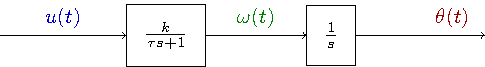
\includegraphics[width=0.8\linewidth]{../../figures/block-DC}
\end{center}
\end{frame}


\begin{frame}[label={sec:org79ab022}]{State-space model with physical states}
\begin{columns}
\begin{column}{0.4\columnwidth}
\begin{center}
  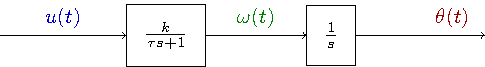
\includegraphics[width=\linewidth]{../../figures/block-DC}
\end{center}

State variables corresponding to physical signals:
\[ x = \begin{bmatrix} x_1\\x_2 \end{bmatrix}= \begin{bmatrix} \omega\\ \theta \end{bmatrix} \]
With dynamics
\begin{align*}
\tau \dot{\omega} &= -\omega + ku\\
\dot{\theta} &= \omega
\end{align*}
\end{column}
\begin{column}{0.4\columnwidth}
\pause

\alert{Activity} Fill the matrix \(A\) and vectors \(B\) and \(C\).

\[ \dot{x} = \begin{bmatrix} \dot{x}_1\\\dot{x}_2\end{bmatrix} = \underbrace{\begin{bmatrix} \textcolor{white}{-\frac{1}{\tau}} & \textcolor{white}{0} \\\textcolor{white}{1} & \textcolor{white}{0} \end{bmatrix}}_{A} \begin{bmatrix} x_1\\x_2\end{bmatrix} + \underbrace{\begin{bmatrix} \textcolor{white}{\frac{k}{\tau}} \\ \textcolor{white}{0} \end{bmatrix}}_{B} u \]
\[ y = \theta = \underbrace{\begin{bmatrix} \textcolor{white}{0} & \textcolor{white}{1} \end{bmatrix}}_{C} \begin{bmatrix} x_1\\x_2\end{bmatrix} \]
\end{column}
\end{columns}
\end{frame}





\begin{frame}[label={sec:org59d2f62}]{State-space model with physical states}
\begin{columns}
\begin{column}{0.4\columnwidth}
\begin{center}
  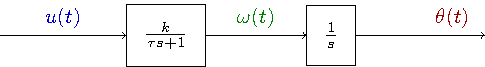
\includegraphics[width=\linewidth]{../../figures/block-DC}
\end{center}

State variables corresponding to physical signals:
\[ x = \begin{bmatrix} x_1\\x_2 \end{bmatrix}= \begin{bmatrix} \omega\\ \theta \end{bmatrix} \]
With dynamics
\begin{align*}
\tau \dot{\omega} &= -\omega + ku\\
\dot{\theta} &= \omega
\end{align*}
\end{column}
\begin{column}{0.4\columnwidth}
\alert{Activity} Fill the matrix \(A\) and vectors \(B\) and \(C\).

\[ \dot{x} = \begin{bmatrix} \dot{x}_1\\\dot{x}_2\end{bmatrix} = \underbrace{\begin{bmatrix} \textcolor{black}{-\frac{1}{\tau}} & \textcolor{black}{0} \\\textcolor{black}{1} & \textcolor{black}{0} \end{bmatrix}}_{A} \begin{bmatrix} x_1\\x_2\end{bmatrix} + \underbrace{\begin{bmatrix} \textcolor{black}{\frac{k}{\tau}} \\ \textcolor{black}{0} \end{bmatrix}}_{B} u \]
\[ y = \theta = \underbrace{\begin{bmatrix} \textcolor{black}{0} & \textcolor{black}{1} \end{bmatrix}}_{C} \begin{bmatrix} x_1\\x_2\end{bmatrix} \]
\end{column}
\end{columns}
\end{frame}


\begin{frame}[label={sec:org655345c}]{State-space model on controllable canonical form}
\begin{columns}
\begin{column}{0.4\columnwidth}
\begin{center}
  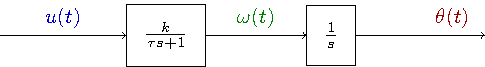
\includegraphics[width=\linewidth]{../../figures/block-DC}
\end{center}

Transfer function
\[G(s) = \frac{ \frac{k}{\tau}} {s( s + \frac{1}{\tau})}\]
\end{column}
\begin{column}{0.6\columnwidth}
The system with transfer function
\begin{equation*}
G(s)=\frac{b_1s^{n-1}+\dots+b_{n-1}s+b_n}{s^n+a_1s^{n-1}+\dots
  +a_{n-1}s+a_n}
\end{equation*}
can be represented on state-space form as
\begin{align*}
\dot{x}&=\bbm -a_1& -a_2& \cdots& -a_{n-1}& -a_n\\
1& 0& \cdots& 0& 0\\
0& 1& \cdots& 0& 0\\
\vdots& \vdots& \ddots& \vdots& \vdots\\
0& 0& \cdots& 1& 0\ebm x+
\bbm 1\\ 0\\ 0\\ \vdots\\ 0\ebm u\\
y&=\bbm b_1& b_2& \cdots& b_n\ebm x
\end{align*}

\pause

\alert{Activity} Determine the state-space model of the DC motor on controllable canonical form
\end{column}
\end{columns}
\end{frame}

\begin{frame}[label={sec:org49ff4e3}]{State-space model on observable canonical form}
\begin{columns}
\begin{column}{0.4\columnwidth}
\begin{center}
  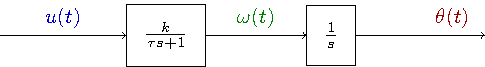
\includegraphics[width=\linewidth]{../../figures/block-DC}
\end{center}

Transfer function
\[G(s) = \frac{ \frac{k}{\tau}} { s(s + \frac{1}{\tau})}\]
\end{column}
\begin{column}{0.6\columnwidth}
The system with transfer function
\begin{equation*}
G(s)=\frac{b_1s^{n-1}+\dots+b_{n-1}s+b_n}{s^n+a_1s^{n-1}+\dots
  +a_{n-1}s+a_n}
\end{equation*}
can be represented on state-space form as
\begin{align*}
\dot{x}&=\bbm -a_1& 1& 0 &\cdots &  0\\
-a_2 & 0& 1 &  \cdots& 0\\
-a_3 & 0 & 0& \cdots & 0\\
\vdots& \vdots& \vdots & \ddots& \vdots\\
-a_n& 0& 0 & \cdots& 0\ebm x+
\bbm b_1\\ b_2\\ b_3\\ \vdots\\ b_n\ebm u\\
y&=\bbm 1& 0& \cdots& 0 \ebm x
\end{align*}

\pause

\alert{Activity} Determine the state-space model of the DC motor on observable canonical form
\end{column}
\end{columns}
\end{frame}

\begin{frame}[label={sec:org45d4d4b}]{State-feedback for model with physical states}
\begin{columns}
\begin{column}{0.4\columnwidth}
\[ \dot{x} = \begin{bmatrix} \dot{x}_1\\\dot{x}_2\end{bmatrix} = \underbrace{\begin{bmatrix} \textcolor{black}{-\frac{1}{\tau}} & \textcolor{black}{0} \\\textcolor{black}{1} & \textcolor{black}{0} \end{bmatrix}}_{A} \begin{bmatrix} x_1\\x_2\end{bmatrix} + \underbrace{\begin{bmatrix} \textcolor{black}{\frac{K}{\tau}} \\ \textcolor{black}{0} \end{bmatrix}}_{B} u \]

Feedback \(u = -\textcolor{morange}{L}x + \textcolor{mbluegreen}{l_0} r\) gives closed-loop system

\begin{align*}
  \dot{x} &= (A-B\textcolor{morange}{L})x + \textcolor{mbluegreen}{l_0}Br\\
  &= \begin{bmatrix} \textcolor{black}{-\frac{1}{\tau}} -\textcolor{morange}{l_1}\frac{k}{\tau} & - \textcolor{morange}{l_2}\frac{k}{\tau} \\\textcolor{black}{1} & \textcolor{black}{0} \end{bmatrix} x + \textcolor{mbluegreen}{l_0} B r
  \end{align*}
with characteristic polynomial
\[s^2 + (\textcolor{black}{\frac{1}{\tau}}  + \textcolor{morange}{l_1}\frac{k}{\tau})s +  \textcolor{morange}{l_2}\frac{k}{\tau} \]
\end{column}


\begin{column}{0.4\columnwidth}
\begin{center}
  \begin{tikzpicture}[scale=0.7]
  \pgfmathsetmacro{\wc}{2}
  \pgfmathsetmacro{\rp}{\wc*cos(45)}
    \draw[->] (-4,0) to (2,0) node[below] {Re};
    \draw[->] (0,-3) to (0,3) node[left] {Im};

    \draw[dashed, black!80] (0,\wc) arc[radius=\wc{}cm, start angle=90, end angle=270]; 

    \node[anchor=center, red!80!black] at (-\rp, \rp) {\Large $\times$ };
    \node[anchor=center, red!80!black] at (-\rp, -\rp) {\Large $\times$ };

    \draw[thin, <->] (0,0) -- node[above] {$\frac{1}{\tau_c}$} (-\rp, \rp);
    \draw[->] (-1, 0) arc[radius=1, start angle=180, end angle=135] node[pos=0.5, left] {\small $45^\circ$};
    \end{tikzpicture}
\end{center}

Desired closed-loop characteristic polynomial

\begin{align*}
  (s-p_1)(s-p_2) &= s^2 + \frac{\sqrt{2}}{\tau_c}s + \frac{1}{\tau_c^2}
\end{align*}
\end{column}
\end{columns}
\end{frame}


\begin{frame}[label={sec:org1eae8d2}]{State-feedback for model with physical states}
Characteristic polynomial obtained with state feedback
\[s^2 + (\textcolor{black}{\frac{1}{\tau}}  + \textcolor{morange}{l_1}\frac{k}{\tau})s +  \textcolor{morange}{l_2}\frac{k}{\tau} \]
Desired characteristic polynomial
\[  s^2 + \frac{\sqrt{2}}{\tau_c}s + \frac{1}{\tau_c^2}\]
\pause

\alert{Activity}
Determine the feedback gains!

\pause
\alert{Solution}
\pause
\begin{align*}
 \textcolor{morange}{l_1} &= \frac{\tau}{k}\big(\frac{\sqrt{2}}{\tau_c} - \frac{1}{\tau}\big) = \frac{\sqrt{2}\tau - \tau_c}{k\tau_c}\\
 \textcolor{morange}{l_2} &= \frac{\tau}{k\tau_c^2} 
\end{align*}
\end{frame}


\begin{frame}[label={sec:org146a8f1}]{Observer for the model with physical states}
\small

\begin{columns}
\begin{column}{0.4\columnwidth}
The observer is given by
     \begin{equation*}
     \begin{split}
     \dot{\hat{x}} &= \underbrace{A \hat{x} + B u{}}_{\text{simulation}} + \underbrace{\textcolor{mred}{K}\big(y - C\hat{x}\big)}_{\text{correction}}\\
&= \left(A - \textcolor{mred}{K}C\right)\hat{x} +  B u{} + \textcolor{mred}{K}y\\
         &= \begin{bmatrix} \textcolor{black}{-\frac{1}{\tau}} & -\textcolor{mred}{k_1}  \\\textcolor{black}{1} & -\textcolor{mred}{k_2}  \end{bmatrix}\hat{x} +  B u{} + \textcolor{mred}{K}y
     \end{split}
     \end{equation*}
with poles given by the eigenvalues of the matrix \(A_o = A - \textcolor{mred}{K}C\),
which has characteristic polynomial
 \begin{equation*}
     \begin{split}
      \det \left( \begin{bmatrix} s & 0\\ 0 & s\end{bmatrix} - \begin{bmatrix} \textcolor{black}{-\frac{1}{\tau}} & - \textcolor{mred}{k_1}  \\\textcolor{black}{1} & -\textcolor{mred}{k_2}\end{bmatrix}\right)\\
= s^2 + (\frac{1}{\tau} + \textcolor{mred}{k_2})s +  (\textcolor{mred}{k_1}+\frac{\textcolor{mred}{k_2}}{\tau})
     \end{split}
     \end{equation*}
\end{column}




\begin{column}{0.4\columnwidth}
\pause

\begin{center}
  \begin{tikzpicture}[scale=0.7]
  \pgfmathsetmacro{\wc}{2}
  \pgfmathsetmacro{\rp}{\wc*cos(45)}
    \draw[->] (-4,0) to (2,0) node[below] {Re};
    \draw[->] (0,-3) to (0,3) node[left] {Im};

    \draw[dashed, black!80] (0,\wc) arc[radius=\wc{}cm, start angle=90, end angle=270]; 

    \node[anchor=center, red!80!black] at (-\rp, \rp) {\Large $\times$ };
    \node[anchor=center, red!80!black] at (-\rp, -\rp) {\Large $\times$ };

    \draw[thin, <->] (0,0) -- node[above] {$\frac{d}{\tau_c}$} (-\rp, \rp);
    \end{tikzpicture}
\end{center}

Choose \(d\) between 2 and 10 and  obtain desired closed-loop characteristic polynomial

\begin{align*}
  (s-p_{o,1})(s-p_{o,2}) &= s^2 + \frac{d\sqrt{2}}{\tau_c}s + \frac{d^2}{\tau_c^2}
\end{align*}
\end{column}
\end{columns}
\end{frame}

\begin{frame}[label={sec:org4823eac}]{Observer for the model with physical states}
Characteristic polynomial of the observer 
\[s^2 + (\frac{1}{\tau} + \textcolor{mred}{k_2})s + (\textcolor{mred}{k_1}+\frac{\textcolor{mred}{k_2}}{\tau})\]
Desired characteristic polynomial
\[  s^2 + \frac{\sqrt{2}d}{\tau_c}s + \frac{d^2}{\tau_c^2}\]
\pause

\alert{Activity}
Determine the observer gains!

\pause
\alert{Solution}
\pause
\begin{align*}
 \textcolor{mred}{k_1} &= \frac{d^2}{\tau_c^2} - \frac{\sqrt{2}d}{\tau_c\tau} + \frac{1}{\tau^2}\\
 \textcolor{mred}{k_2} &= \frac{\sqrt{2}d}{\tau_c} - \frac{1}{\tau} 
\end{align*}
\end{frame}
\end{document}